\documentclass{beamer}

\usepackage{pgfpages}
% \setbeameroption{show notes on second screen}


% Note rendering settings
% \setbeameroption{hide notes} % Default
% \setbeameroption{show notes}
% \setbeameroption{show only notes}

% % \textcolor
\usepackage{xcolor}

% Maths
\usepackage{mathabx}
\usepackage{mathtools}

% Algorithms using algorithmicx package (with its algpseudocode command set)
\usepackage{algpseudocode}

% Operators for common operations
\DeclareMathOperator{\DFT}{DFT}
\DeclareMathOperator{\DWT}{DWT}
\DeclareMathOperator{\FFT}{FFT}

% Code listings
\usepackage{listings}
\usepackage{lstautogobble}
\lstset{
		basicstyle=\small,
		breaklines=true,
		autogobble=true,
		postbreak=\mbox{$\drsh$},
}

% Date management
\usepackage{datetime2}
\DTMsavedate{presentation}{2021-12-14}

% BibLaTeX
\usepackage[
  style=alphabetic,
  backend=biber, % Default backend, just listed for completness
  sorting=ynt % Sort by year, name, title
]{biblatex}
\addbibresource{references.bib}
\nocite{*}

% User numeric labels (instead of icons) in bibliography page
\setbeamertemplate{bibliography item}{\insertbiblabel}

% Somber theme with right-justified headings
\usetheme{Pittsburgh}

% Red colour for headings
% \usecolortheme{beaver}

% Rectangles (instead of ugly dots) for enumeration bullet points
\useinnertheme{rectangles}

% Gray (instead of the default blue) for bullet points
% \setbeamercolor{itemize item}{fg=gray}
% \setbeamercolor{itemize subitem}{fg=gray}

\title{Schönhage–Strassen Algorithm for Fast Multiplication}

\author{Michael Senn}
\institute{Faculty of Science, University of Bern}
\date{\DTMusedate{presentation}}

\begin{document}
\begin{frame}
		\titlepage

		\note[item]{Welcome to my presentation for this seminar, we'll be talking about ...}
\end{frame}

% Only show sections
\setcounter{tocdepth}{1}
\begin{frame}
		\frametitle{Outline}
		\frametitle{\secname}
		\framesubtitle{\subsecname}
		\tableofcontents
		\note{Will introduce the problem, and outline some earlier methods}
		\note{Briefly explain mathematical concepts of DFT and convolution theory}
		\note{Moving on to using the FFT for fast multiplication}
		\note{Culminating in the Schönhage-Strassen algorithm}
\end{frame}

\section{Introduction}

\begin{frame}
		\frametitle{\secname}

		\textbf{Goal: Multiplying large integers}

		\begin{itemize}
				\item Given $x, y$ two $n$-bit integers
				\item Where $x = x_0, x_1, \ldots, x_{n-1}$, $y = y_0, y_1, \ldots, y_{n-1}$ big-endian representation
				\item Calculate $z \coloneqq x \cdot y$
		\end{itemize}
\end{frame}

\subsection{Long multiplication}

\begin{frame}
		\frametitle{\secname}
		\framesubtitle{\subsecname}

		\begin{itemize}
				\item Multiply digit by digit, sum up the products
				\item Complexity: $O(n^2)$ additions and multiplications
				\item Up to 1960: Long multiplication conjectured to be asymptotically optimal
				\item We can do better
		\end{itemize}
\end{frame}

\subsection{Karatsuba algorithm}

\begin{frame}
		\frametitle{\secname}
		\framesubtitle{\subsecname}

		\begin{itemize}
				\item Anatoly Karatsuba, 1960
				\item Idea: Work in large base $W$
				\item $x = x_0 + x_1 \cdot W$, where $x_0, x_1 \in [0, W - 1]$
				\item Karatsuba relation
						\begin{align*}
								xy & = \frac{t + u}{2} - v + \frac{t - u}{2} \cdot W + v \cdot W^2 \\ 
								t & = (x_0 + x_1) \cdot (y_0 + y_1) \\
								u & = (x_0 - x_1) \cdot (y_0 - y_1) \\
								v & = x_1 \cdot y_1
						\end{align*}
				\item Replaces one multiplication of two $2n$-digit numbers
						with three multiplications of $n$-digit numbers
				\item Divide and conquer: Asymptotic complexity of
						$O(n^{\log_2{3}}) \approx O(n^{1.58})$
		\end{itemize}
\end{frame}

\subsection{Toom-Cook method}

\begin{frame}
		\frametitle{\secname}
		\framesubtitle{\subsecname}

		\begin{itemize}
				\item Toom 1963, Cook 1966
				\item Idea: Interpret digits of $x$ and $y$ as coefficients of polynomial of degree $D - 1$
				\item $x(t) = x_0 + x_1 \cdot t + \ldots + x_{D-1} \cdot t^{D-1}$
				\item $z(t) \coloneqq x(t) \cdot y(t)$ has degree $2D - 2$
				\item Evaluate $z(t)$ at $2D - 1$ values
				\item Reconstruct coefficients of polynomial $z(t)$
				\item For $D = 3$, asymptotic complexity of $\approx O(n^{1.46})$
		\end{itemize}
\end{frame}

\section{Discrete Fourier Transform (DFT)}

\begin{frame}
		\frametitle{\secname}

		\textbf{Goal}: Perform Fourier analysis of discrete signal $x = (x_0,
		x_1, \ldots, x_{n-1})$ in some algebraic field.
		\note{Usual definition over field of complex numbers. We will (later) use it over a finite field}

		\begin{align*}
				\DFT(x): X_k & = \sum_{j=0}^{n-1} x_j \cdot g^{-j k} \\
				\DFT^{-1}(X): x_j & = \frac{1}{n} \sum_{k=0}^{n-1} X_k \cdot g^{j k}
		\end{align*}

		Where $g$ is a primitive $n$-th root of unity (i.e. $g^n = 1$, $g^m
		\neq 1 \forall m < n$)
\end{frame}

\subsection{Calculating the DFT}

\begin{frame}
		\frametitle{\secname}
		\framesubtitle{\subsecname}

		\begin{itemize}
				\item Naive approach would be $O(n^2)$
				\item Recall first presentation: FFT algorithm allows calculation in $O(n \log(n))$
				\item We'll use FFT as blackbox: $\FFT(x) = \DFT(x)$.
		\end{itemize}
\end{frame}

\section{Convolution theory}

\begin{frame}
		\frametitle{\secname}

		Given two signals $f$ and $g$, their convolution is defined as:
		\[
				(f * g)(t) \coloneqq \int_{-\infty}^{\infty} f(\tau) \cdot g(t - \tau) d\tau
		\]

		\note{Applications in signal \& image processing, computer vision, pure mathematics, ...}
		
		\textbf{However} we work with finite signals. We introduce four types
		of discrete convolution operations. Consider finite signals $x, y$
\end{frame}

\subsection{Cyclic convolution}

\begin{frame}
		\frametitle{\secname}
		\framesubtitle{\subsecname}

 		\begin{columns}
 				\column{0.5\textwidth}
				\textbf{Cyclic} convolution $z = x \times y$ is $n$-length discrete
				signal with components:
				\[
						z_k \coloneqq \sum_{i + j \equiv k \pmod{n}} x_i \cdot y_j
				\]
				\note{Symmetry is result of commutativity in field}
 				\column{0.5\textwidth}
 				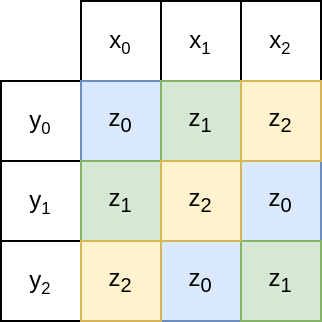
\includegraphics[width=\textwidth]{../resources/cyclic_convolution.drawio.png}
		\end{columns}
\end{frame}

\subsection{Acyclic convolution}

\begin{frame}
		\frametitle{\secname}
		\framesubtitle{\subsecname}

 		\begin{columns}
 				\column{0.5\textwidth}
				\textbf{Acyclic} convolution $u = x \times_A y$ is $2n$-length discrete
				signal with components:
				\note{Observe: Acyclic separates cylic into those where addition `wrapped around' vs those where it didn't}
				\begin{align*}
						u_k & \coloneqq \sum_{i + j = n} x_i \cdot y_j \\
						u_{2n - 1} & \coloneqq 0
				\end{align*}
 				\column{0.5\textwidth}
 				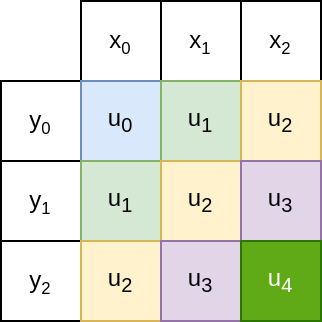
\includegraphics[width=\textwidth]{../resources/acyclic_convolution.drawio.png}
		\end{columns}
\end{frame}

\subsection{Negacyclic convolution}

\begin{frame}
		\frametitle{\secname}
		\framesubtitle{\subsecname}

 		\begin{columns}
 				\column{0.5\textwidth}
				\textbf{Negacyclic} convolution $v = x \times_\_ y$ is $n$-length discrete
				signal with components:
				\[
						v_k \coloneqq \sum_{i + j = n} x_i \cdot y_j - \sum_{i + j = n + k} x_i \cdot y_j
				\]
 				\column{0.5\textwidth}
 				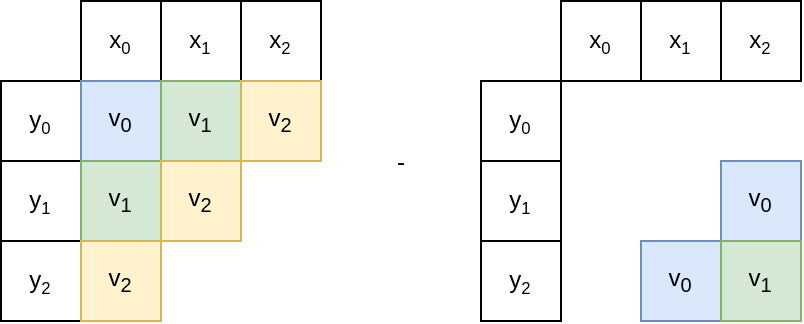
\includegraphics[width=\textwidth]{../resources/negacyclic_convolution.drawio.png}
		\end{columns}
\end{frame}

\subsection{Half-cyclic convolution}

\begin{frame}
		\frametitle{\secname}
		\framesubtitle{\subsecname}

 		\begin{columns}
 				\column{0.5\textwidth}
				\textbf{Half-cyclic} convolution $w = x \times_H y$ is $n$-length discrete
				signal with first $n$ components of acyclic convolution $x \times_A y$:
				\[
						w_k \coloneqq (x \times_A y)(k)
				\]
 				\column{0.5\textwidth}
 				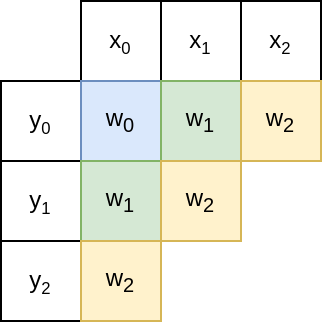
\includegraphics[width=\textwidth]{../resources/halfcyclic_convolution.drawio.png}
		\end{columns}
\end{frame}

\subsection{Relation between convolutions}

\begin{frame}
		\frametitle{\secname}
		\framesubtitle{\subsecname}

		Convolutions are related. Being able to e.g. calculate cyclic and
		negacyclic allows to also calculate half-cyclic or acyclic
		convolutions.

		\begin{align*}
				x \times_H y & = \frac{1}{2} \cdot ((x \times y) + (x \times_{\_} y)) \\
				x \times_A y & = (x \times_H y) || \frac{1}{2} \cdot ((x \times y) - (x \times_{\_} y)) \\
				L(x) \times_A L(y) & = x \times y = x \times_{\_} y\text{, where } n = 2k, x_i = y_i = 0 \forall i \geq k
		\end{align*}
		\note{$L$ here is left half of signal of length $2n$}
\end{frame}

\subsection{Convolution theorem}

\begin{frame}
		\frametitle{\secname}
		\framesubtitle{\subsecname}

		\note{Now we want to tie together convolutions and DFT}

		We can calculate the cyclic convolution using the DFT:
		\[
				x \times y = \DFT^{-1}(\DFT(x) \cdot \DFT(y))
		\]

		\note{The multiplication here is component-wise multiplication}

		This is $O(n \log n)$ instead of the naive $O(n^2)$ if using the FFT.
\end{frame}

\subsection{Multiplication is a type of convolution!}

\begin{frame}
		\frametitle{\secname}
		\framesubtitle{\subsecname}

		\note{Why do we care about convolutions?}

		Consider long multiplication with a delayed carry operation.
		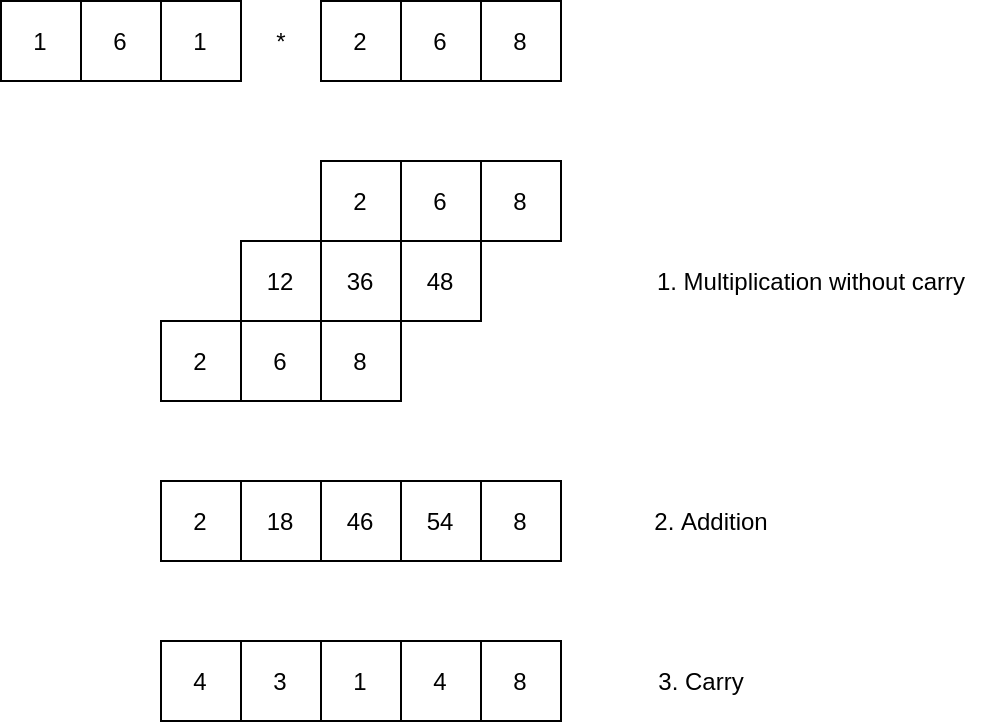
\includegraphics[width=0.7\textwidth]{../resources/long_multiplication.drawio.png}
\end{frame}

\begin{frame}
		\frametitle{\secname}
		\framesubtitle{\subsecname}

		The multiplication part is an acyclic convolution.
		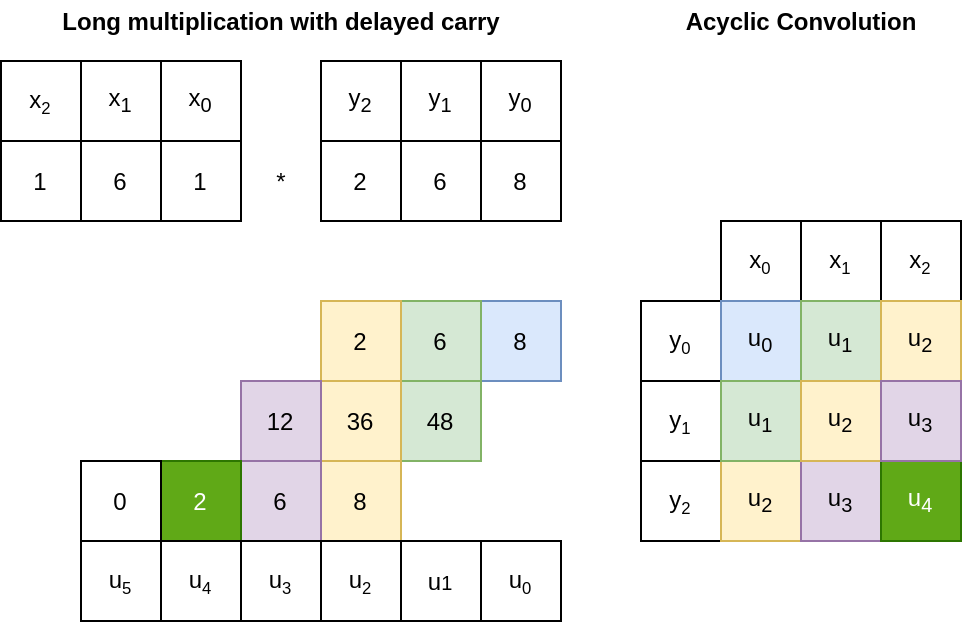
\includegraphics[width=0.7\textwidth]{../resources/multiplication_convolution.drawio.png}
\end{frame}

\section{FFT Multiplication}

\begin{frame}
		\frametitle{\secname}

		Given $x, y$ two $n$-digit integers in base $B$, start by zero-padding.

		\begin{algorithmic}[1]
				\Function{FFTMult}{$x, y$} \Comment{$x, y$ $n$-digit base-$B$ integers}
				\State $x \gets$ \Call{Pad}{x, 2n} \Comment{Zero-pad to length $2n$ on right side}
				\State $y \gets$ \Call{Pad}{y, 2n}
				\algstore{fftmult}
		\end{algorithmic}
\end{frame}

\begin{frame}
		\frametitle{\secname}

		Calculate the acyclic convolution $x \times_A y$ by means of the
		convolution theorem. Mind that we must round the results, as we might
		be in an arbitrary field such as the field of complex numbers!

		\begin{algorithmic}[1]
				\algrestore{fftmult}
				\State $X \gets$ \Call{DFT}{x}
				\State $Y \gets$ \Call{DFT}{y}
				\\
				\State $Z \gets X \cdot Y$ \Comment{Dyadic product}
				\\
				\State $z \gets$ $\Call{DFT}{Z}^{-1}$
				\State $z \gets$ \Call{round}{z}
				\algstore{fftmult}
		\end{algorithmic}
\end{frame}

\begin{frame}
		\frametitle{\secname}

		Finally perform the carry operation and return the result.

		\begin{algorithmic}[1]
				\algrestore{fftmult}
				\State $carry \gets 0$
				\For{$i \gets 0$ to $2n$}
				  \State $v \gets z_i + carry$
				  \State $z_n \gets v \mod B$
				  \State $carry \gets v / B$ \Comment{Integer division}
				\EndFor
				\State \textbf{Return} $z_0 || z_1 || \ldots || z_n || carry$ \Comment{Optionally remove high-order 0s}
				\EndFunction
		\end{algorithmic}
\end{frame}

\section{Schönhage-Strassen algorithm}

\begin{frame}
		\frametitle{\secname}

		\textbf{Goal}: Work in a more convenient algebraic domain than the
		field of complex numbers.

		Transform the signal components into elements of the ring
		$\mathbb{Z}_{2^m + 1}$. Then:

		\begin{itemize}
				\item No rounding problems
				\item Integer operations more performant than floating-point
						operations
				\item Multiplication and division by multiples of two can be
						optimized further
		\end{itemize}

\end{frame}

\subsection{Discrete Weighted Transform (DWT)}

\begin{frame}
		\frametitle{\secname}
		\framesubtitle{\subsecname}

		Let $x, a$ be length-$n$ signals. Then we define the \textbf{discrete weighted transform}:
		\begin{align*}
				\DWT(x, a) : X_k & = \sum_{j=0}^{n-1} (a_j \cdot x_j) \cdot g^{-jk} \\
				\DWT^{-1}(X, a) : x_j & = \frac{1}{n a_j} \cdot \sum_{k = 0}^{n - 1} X_k \cdot g^{jk}
		\end{align*}

		It is clear that:
		\begin{align*}
				\DWT(x, a) = \DFT(x \cdot a)
		\end{align*}
\end{frame}

\subsection{Weighted cyclic convolution}

\begin{frame}
		\frametitle{\secname}
		\framesubtitle{\subsecname}

		Given a weight vector $a$, the \textbf{weighted cyclic} convolution $z
		= x \times_a y$ is $n$-length discrete signal with components:
		\[
				z_k \coloneqq \frac{1}{a_k} \sum_{i + j \equiv k \pmod{n}} (x_i \cdot a_i) \cdot (y_j \cdot a_j)
		\]
\end{frame}

\subsection{Weighted convolution theorem}

\begin{frame}
		\frametitle{\secname}
		\framesubtitle{\subsecname}

		Recall the convolution theorem which allowed to calculate a cyclic
		convolution using the DFT. Equivalently, the DWT can be used to
		calculate the weighted cyclic convolution:
		\[
				x \times_a y = \DWT^{-1}(\DWT(x, a) \cdot \DWT(y, a), a)
		\]

		We can use this --- with an appropriate weight vector $a$ --- to
		calculate \textbf{other} convolutions. Let $A$ be a primitive $2n$-th
		root of unity, $a = (A^j)$ then:
		\begin{align*}
				x \times_{\_} y & = x \times_a y
		\end{align*}
\end{frame}

\subsection{Core idea}

\begin{frame}
		\frametitle{\secname}
		\framesubtitle{\subsecname}

		Core idae of Schönhage-Strassen: Work in $\mathbb{Z} / N \mathbb{Z}$,
		where $N = 2^n + 1$ for an integer $n$. Then choose $D = 2^k$ such that
		$D | n$ to be the number of parts into which we split our numbers. Then:

		\begin{itemize}
				% \item Any positive integer $x < F_n$ can be (non-uniquely)
				% 		represented as a $2^n + 1$ bit string
				\item Reduction modulo $2^n + 1$ can be done efficiently
				\item Primtive roots of unity have the form $2^k$, allowing for
						efficient operations
				\note{In fact, $2$ is a $2^{n+1}$-th primitive root of unity.}
		\end{itemize}

		% The core idea of Schönhage-Strassen is to choose a modulus of a Ferma prime $F_n = 2^{2^{n}} + 1$$N = 2^n +
		% 1$, such that $P = 2^p | n$, where $P$ will be the number of parts into
		% which we split our input.
\end{frame}


\subsection{Algorithm}

\begin{frame}
		\frametitle{\secname}
		\framesubtitle{\subsecname}

		Consider two integers $0 \leq x, y < 2^n + 1$.

		\begin{algorithmic}[1]
				\Function{Schönhage-Strasse-Mult}{$x, y$}
				\State $D \gets 2^k$ such that $D | n$
				\State $M \gets 2^l$ such that $DM = n$
				\State Pick smallest $n' \geq 2M + k$ such that $n' = DM'$
				\algstore{ssmult}
		\end{algorithmic}

		$n'$ chosen to be large enough to accomodate largest possible element
		of convolution, yet small enough ($n' < n$) so that recursion makes
		progress.
\end{frame}

\begin{frame}
		\frametitle{\secname}
		\framesubtitle{\subsecname}

		Split the input numbers into $D$ parts of $M$ bits each.
		\note{Split input signal is now a base-$2M$ representation of the original number}

		\begin{algorithmic}[1]
				\algrestore{ssmult}
				\State $X \gets $\Call{Split}{x, D}
				\State $Y \gets $\Call{Split}{y, D}
				\algstore{ssmult}
		\end{algorithmic}
\end{frame}

\begin{frame}
		\frametitle{\secname}
		\framesubtitle{\subsecname}

		Calculate the DWT using appropriate weight vectors. Recall that
		multiplication with roots of unity can be done efficiently.

		\begin{algorithmic}[1]
				\algrestore{ssmult}
				\For{$i \gets 0, D$}
				\State $X_i \gets (2^{jM'} X_i) \bmod (2^{n'} + 1)$
				\State $Y_i \gets (2^{jM'} Y_i) \bmod (2^{n'} + 1)$
				\EndFor
				\\
				\State $X \gets$ \Call{DFT}{X}
				\State $Y \gets$ \Call{DFT}{Y}
				\algstore{ssmult}
		\end{algorithmic}

		\[
				x \times_a y = \DWT^{-1}({\color{red}\DWT(x, a)} \cdot {\color{red}\DWT(y, a)}, a)
		\]
\end{frame}

\begin{frame}
		\frametitle{\secname}
		\framesubtitle{\subsecname}

		Dyadic multiplication stage. These multiplications can be done
		recursively, or with any other multiplication algorithm.

		\begin{algorithmic}[1]
				\algrestore{ssmult}
				\For{$i \gets 0, D$}
				\State $X_i \gets X_i Y_i \bmod(2^{n'} + 1)$
				\EndFor
				\algstore{ssmult}
		\end{algorithmic}

		\[
				x \times_a y = \DWT^{-1}(\DWT(x, a) {\color{red}\cdot} \DWT(y, a), a)
		\]
\end{frame}

\begin{frame}
		\frametitle{\secname}
		\framesubtitle{\subsecname}

		Calculate the inverse discrete weighted transform.

		\begin{algorithmic}[1]
				\algrestore{ssmult}
				\State $X \gets$ \Call{DFT}{A}

				\For{$i \gets 0, D$}
				\State $Z_i \gets X_{D - i} / 2^{k + jM'} \bmod (2^{n'} + 1)$
				\algstore{ssmult}
		\end{algorithmic}

		Observe how, rather than calculating the inverse DFT directly, this
		calculates it by means of the DFT and then switching the order of the
		output signal's components, as shown by Duhamel et
		al\autocite{duhamelComputingInverseDFT1988}.

		\[
				x \times_a y = {\color{red}\DWT^{-1}}(\DWT(x, a) \cdot \DWT(y, a), a)
		\]
\end{frame}

\begin{frame}
		\frametitle{\secname}
		\framesubtitle{\subsecname}

		Adjust sign if value $Z_i$ exceeds largest possible value $(i + 1)
		\cdot 2^{2N / 2^k}$ of $i$-th element.

		\begin{algorithmic}[1]
				\algrestore{ssmult}
				\If{$Z_i > (i + 1) \cdot 2^{2M}$}
				\State $Z_i \gets Z_i - (2^{n'} + 1)$
				\EndIf
				\EndFor
				\algstore{ssmult}
		\end{algorithmic}
\end{frame}

\begin{frame}
		\frametitle{\secname}
		\framesubtitle{\subsecname}

		Perform carry operation

		\begin{algorithmic}[1]
				\algrestore{ssmult}
				\State $carry \gets 0$
				\For{$i \gets 0$ to $D$}
				  \State $v \gets Z_i + carry$
				  \State $Z_i \gets v \mod 2^M$
				  \State $carry \gets v / 2^M$ \Comment{Integer division}
				\EndFor
				\If{$carry > 0$}
				\State Include $carry$ as high-order word $Z_{D+1}$
				\EndIf
				\algstore{ssmult}
		\end{algorithmic}
\end{frame}

\begin{frame}
		\frametitle{\secname}
		\framesubtitle{\subsecname}

		Finally returning the product $x \cdot y \bmod 2^n + 1$.

		\begin{algorithmic}[1]
				\algrestore{ssmult}
				\State \textbf{Return} $\{Z_0, Z_1, \ldots, Z_{D+1}\}$ \Comment{Product in base $2^M$}
				\EndFunction
		\end{algorithmic}
\end{frame}

\subsection{Complexity}

\begin{frame}
		\frametitle{\secname}
		\framesubtitle{\subsecname}

		Analysis shows that the Schönhage-Strassen algorithm has an asymptotic
		complexity of
		\[
				O(n \cdot \log(n) \cdot \log(\log(n)))
		\]

		Schönhage and Strassen conjecture that an optimal complexity for integer multiplication of
		\[
				O(n \cdot \log(n))
		\]
		can be achieved.


\end{frame}

\section{Summary}

\begin{frame}
		\frametitle{\secname}

		We have seen:
		\begin{itemize}
				\item How to model an integer multiplication as an acyclic convolution
				\item How to express convolutions as a sequence of DFT, DWT and dyadic products
				\item How to efficiently calcualte the DFT and DWT using the FFT
				\item How to transform the work into a domain where many of the
						operations are much more efficient
		\end{itemize}
\end{frame}

\section{References}

\begin{frame}[allowframebreaks]
		\frametitle{References}
		\printbibliography
\end{frame}

\end{document}
